% -*-coding: utf-8-*-

\startconclusionpage
	Описанные инструменты в данной работе были успешно реализованы и использованы в компании ООО «Научно-Технический Центр ПРОТЕЙ». Применился в проекте GGSN \cite{ggsn}, одной из его функций является маршрутизацией пользовательского трафика. Для каждого абонента заводились различные таймера, по истечении которых происходили определенные действия: например запрос на удаление пользователя (DELETE PDP CONTEXT REQUEST), либо отправление запроса на обновление используемых данных в RADIUS \cite{radius} сервер. Так как абонентов большое количество, требовалась реализация таймеров с высокой производительностью. Таймеры были взяты из набора библиотек DPDK \cite{dpdk}, они реализованы с помощью структуры данных - список с пропусками \cite{skip_list}. При тестировании проекта были обнаружены замедления. Благодаря написанному профайлеру стало известно, что замедление происходило из-за таймеров. На рисунке \ref{fig:slow_timers_profile} показан профиль приложения, в котором была вынесена отдельная работа с таймерами.
    \begin{figure}[H]
        \caption{профиль приложения работающего с таймерами из DPDK}
        \label{fig:slow_timers_profile}
        \centering
        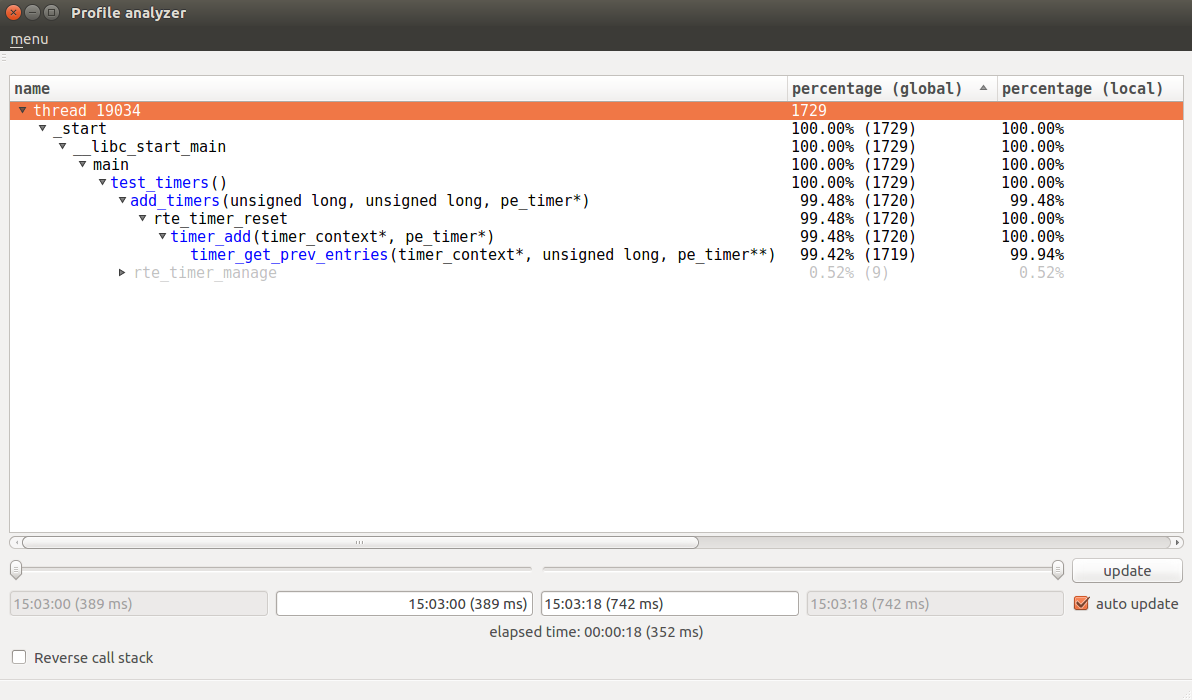
\includegraphics[scale=0.4]{images/slow_timers_profile}
    \end{figure}    
    
    Из профиля видно, что большую часть времени занимает добавление нового таймера. Хотя добавление имеет такую же сложность как и функция поиска истекших таймеров (на рисунке это \verb|rte_timer_manage|). При дальнейшем анализе обнаружилась ошибка в библиотеке, которая возникала из-за удаления ссылок на старших уровнях списка с пропусками, при срабатывании таймера который не был расположен на них. Из-за этого асимптотика работы добавления таймера  начинала занимать $O($количества добавленных таймеров$)$, т.е. сложность была линейной, а не логарифмической. Исправление ошибки заметно ускорило приложение.    
    
    Написанный профайлер также успешно использовался при оптимизации себя же. Благодаря ему были выявлены узкие места в инструменте для визуализации данных, исправление которых ускорило его. Проблема была в использовании функции \verb|sscanf| при считывании символов записанных в файл после работы инструмента по сбору данных. Оказалось, что она внутри вызывает подобие \verb|strlen| которая считает длину буфера, пробегая по нему в поисках \verb|\0|. В файле было записано много строк, содержащих адрес на начало функции, размер ее и имя функции. После прочтения одной строчки, указатель на начало буфера сдвигался на размер строки и разбор файла продолжался дальше. Так как такая строчка занимает не больше 1000 символов, то \verb|sscanf| вызывался $O($размера буффера$)$ раз. В итоге получилось, что функция разбора символов работала за $O(($размер буффера$) ^ 2)$. Замена \verb|sscanf| на самописную функцию дало ускорение, т.е. разбор файла стал работать за $O($размер буффера$)$. Также был оптимизирован инструмент для сбора информации, в котором происходило постоянное сбрасывание буфера при создании файла с данными, что было обнаружено благодаря написанному профайлеру. %% Успешно применился и помог ускорить решения написанные в нашей компании.
    
    В дальнейшем планируется добавить возможность профилировать в реальном времени. Для этого нужен будет агент, который будет запускаться на удаленной машине, с возможность подключения к нему. Также планируется расширить его с добавлением возможности визуализировать пользовательские данные в зависимости от времени. Еще остается вопрос производительности, планируется уменьшить накладные расходы профайлера на приложение.
	

\printmainbibliography

%% После этой команды chapter будет генерировать приложения, нумерованные русскими буквами.
%% \startappendices из старого стилевика будет делать то же самое
\appendix

\chapter{Измерение времени работы}

Здесь будут показаны несколько различных программ на которых проводилось исследование накладных расходов,  появляющихся в результате работы профайлера.

\lstinputlisting[label=code:logger,caption=Исходный код программы для логирования]{appendix/logger.tex}

\lstinputlisting[label=code:writer,caption=Исходный код программы записывающей различные значения]{appendix/writer.tex}

























% В приложениях рисунки, таблицы и другие подобные элементы нумеруются по приложениям с соответствующим префиксом. Проверим это.

% Листинг~\ref{lst4:apx} должен иметь номер А.1.

% \begin{algorithm}[!h]
% \caption{Исходный код и флоат \texttt{algorithm}}\label{lst4:apx}
% \begin{lstlisting}
% public class HelloWorld {
% 	public static void main(String[] args) {
% 		System.out.println("Hello, world!");
% 	}
% }
% \end{lstlisting}
% \end{algorithm}

% Рисунок~\ref{fig2:apx} должен иметь номер A.1.

% \begin{figure}[!h]
% \caption{Пример рисунка}\label{fig2:apx}
% \centering
% \begin{tikzpicture}[scale=0.7]
% \draw[thick,->] (0,0)--(3.5,0);
% \draw[thick,->] (0,0)--(0,3.5);
% \draw[very thick, red] (0,0)--(3,3);
% \draw[dashed] (3,0)--(3,3);
% \draw[dashed] (1.5,0)--(1.5,1.5);
% \end{tikzpicture}
% \end{figure}

% Таблица~\ref{tab3:apx} должна иметь номер A.1.

% \begin{table}[!h]
% \caption{Таблица умножения с помощью \texttt{tabu} (фрагмент)}\label{tab3:apx}
% \centering
% \begin{tabu}{|*{18}{X[c]|}}\hline
% -- & 1 & 2 & 3 & 4 & 5 & 6 & 7 & 8 & 9 & 10 & 11 & 12 & 13 & 14 & 15 & 16 & 17 \\\hline
% 1  & 1 & 2 & 3 & 4 & 5 & 6 & 7 & 8 & 9 & 10 & 11 & 12 & 13 & 14 & 15 & 16 & 17 \\\hline
% 2  & 2 & 4 & 6 & 8 & 10 & 12 & 14 & 16 & 18 & 20 & 22 & 24 & 26 & 28 & 30 & 32 & 34 \\\hline
% 3  & 3 & 6 & 9 & 12 & 15 & 18 & 21 & 24 & 27 & 30 & 33 & 36 & 39 & 42 & 45 & 48 & 51 \\\hline
% 4  & 4 & 8 & 12 & 16 & 20 & 24 & 28 & 32 & 36 & 40 & 44 & 48 & 52 & 56 & 60 & 64 & 68 \\\hline
% \end{tabu}
% \end{table}

% Заодно проверим нумерованные и ненумерованные перечисления. Ненумерованные:
% \begin{itemize}
%     \item пункт А;
%     \item пункт Б;
%     \item пункт В.
% \end{itemize}

% Нумерованные списки нескольких уровней:
% \begin{enumerate}
%     \item первый элемент;
%     \item второй элемент с подэлементами:
%     \begin{enumerate}
%         \item первый подэлемент;
%         \item второй подэлемент;
%         \item третий подэлемент.
%     \end{enumerate}
%     \item третий элемент;
%     \item четвертый элемент;
%     \item пятый элемент;
%     \item шестой элемент;
%     \item седьмой элемент;
%     \item восьмой элемент;
%     \item девятый элемент;
%     \item десятый элемент.
% \end{enumerate}

% \chapter{Еще один пример приложения  с неимоверно длиннющим названием для тестирования переносов}

% Проверим на примере таблиц, что нумерация в приложениях~--- по приложениям.
% Таблица~\ref{tab3:apx2} должна иметь номер Б.1.

% \begin{table}[!h]
% \caption{Таблица умножения с помощью \texttt{tabu} (фрагмент)}\label{tab3:apx2}
% \centering
% \begin{tabu}{|*{18}{X[c]|}}\hline
% -- & 1 & 2 & 3 & 4 & 5 & 6 & 7 & 8 & 9 & 10 & 11 & 12 & 13 & 14 & 15 & 16 & 17 \\\hline
% 1  & 1 & 2 & 3 & 4 & 5 & 6 & 7 & 8 & 9 & 10 & 11 & 12 & 13 & 14 & 15 & 16 & 17 \\\hline
% 2  & 2 & 4 & 6 & 8 & 10 & 12 & 14 & 16 & 18 & 20 & 22 & 24 & 26 & 28 & 30 & 32 & 34 \\\hline
% 3  & 3 & 6 & 9 & 12 & 15 & 18 & 21 & 24 & 27 & 30 & 33 & 36 & 39 & 42 & 45 & 48 & 51 \\\hline
% 4  & 4 & 8 & 12 & 16 & 20 & 24 & 28 & 32 & 36 & 40 & 44 & 48 & 52 & 56 & 60 & 64 & 68 \\\hline
% \end{tabu}
% \end{table}
